\chapter{Event selection}
The event selection has been optimized in order to maximize the significance of the signal over backgraound.
The whole event selection of the analysis is shown in this chapter.

%overview
First the preselection cuts are applied including basic event cleaning and the trigger requirements, then the specific event selection is applied to the each 0,1,2-lepton channels.
For the main event selection, first the selection of the one $W/Z$ boson decaying leptonically is selected. Then in each channel, the forward jets and the hadronically decaying boson is selected and the Signal region (SR) and the Control region (CR) is defined, finally the selection to enhance the VBS topology is applied before using the machine learning approach to get the final discriminant.
%merged and resolved region 
The events are categorized into two regions depends on the type of the jets included. The events has one or more large-R jets are categorized as merged region, otherwise resolved region. In the merged region, forward jets are selected by choosing two small-R jets with the highest invariant mass ($m_{jj}^{tag}$), then the large-R jet with the highest $p_T$ is chosed as the merged jets decayed from $W/Z$ boson $(V_{had})$. In the resolved region, forward jets are selected same as in the merged region, then two jets with the higest and the second highest $p_T$ is selected from the rest of the small-R jets as the jets decaying from $V_{had}$.

Further details are shown hereafter.

\section{Common selection}
The selection of the $W/Z$ boson decaying leptonically is applied before categorizing of the signal region (SR) and the control region (CR) is described here. \\
\noindent \textbf{0-lepton}\\
The $Z \rightarrow \nu\nu$ identification requires no Loose lepton and high missing energy (E$_T^{miss}$ > 200~GeV) in the final state. There are significant QCD multijet background in 0-lepton channel, therefore some cuts suppressing the multijets are applied: \\
\\
- $p_{\mathrm{T}}^{\mathrm{miss}}>50 \mathrm{GeV}$ \\
- $\Delta \phi\left(E_{\mathrm{T}}^{\mathrm{miss}}, p_{\mathrm{T}}^{\mathrm{miss}}\right)<\pi / 2$ \\
- $\min \left(\Delta \phi\left(E_{\mathrm{T}}^{\mathrm{miss}}, j\right)\right)>\pi / 6$ \\
- $\Delta \phi\left(E_{\mathrm{T}}^{\mathrm{miss}}, \overrightarrow{\mathbf{V}}_{\mathrm{had}}\right)>\pi / 9$ \\ \\
where $p_{\mathrm{T}}^{\mathrm{miss}}$ is the track-based missing momentum, and $\min \left(\Delta \phi\left(E_{\mathrm{T}}^{\mathrm{miss}}, j\right)\right)$ is the minimum azimuthal difference betwween $E_{\mathrm{T}}^{\mathrm{miss}}$ and small-R jets. \\

\noindent\textbf{1-lepton} \\
To select the events with $W \rightarrow l\nu$ candidate, exactly one Tight lepton is required.
In order to suppress the multi-jet background, following cuts are applied for all regions: \\ \\
- $E_{\mathrm{T}}^{\text {miss }}>80 \mathrm{GeV}$ \\ 
- $p_{\mathrm{T}, \ell}>28 \mathrm{GeV}$ \\
- $m_{J}>50 \mathrm{GeV}$ (merged only) \\ \\

\noindent\textbf{2-lepton} \\
The $Z \rightarrow ll$ candidates are selected by requiring two isolated same-flavour Loose leptons. Both leptons required to be $p_T$ > 27~GeV. Opposite charges are required only for muons and not for electrons, since electrons are more sensitive to charge mis-identification due to the conversions of photons from bremsstrahlung, especially at high $E_T$.
The $m_{ll}$, invariant mass of the dilepton is required to be in the mass window \\ \\
- $83 < m_{ee}< 99~GeV$ \\ 
- $\left(85.6-0.0117 p_{\mathrm{T}, \ell \ell}\right)<m_{\mu \mu}<\left(94.0+0.0185 p_{\mathrm{T}, \ell \ell}\right) \mathrm{GeV}$ \\ \\
The second equation for muons was oprimized from the 2015+16 analysis~\cite{}. 
The modeling distribution of lepton distribution in the early stage of the selection is shown in Figure~\ref{fig:2lepLeptons}. The mass peak of Z boson can be seen here.

\begin{figure}[ht]
    \centering
    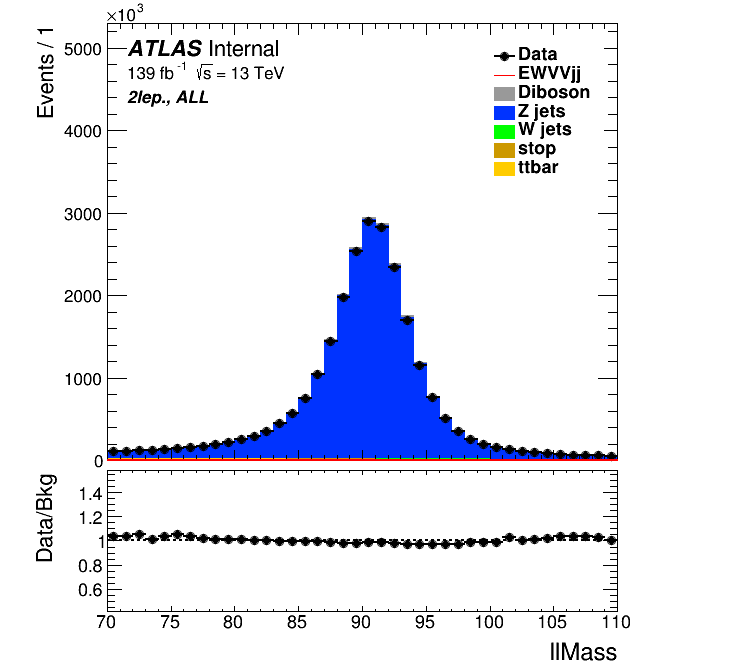
\includegraphics[width=0.5\textwidth]{figures/2lep/dataMC/C_0ptag1pfat0pjet_0ptv_ALL_llMass_Lin.png}
    \caption{Lepton distributions in 2-lepton channel. The events before any selections are shown. Z mass peak is shown in $M_{ll}$ distribution.}
    \label{fig:2lepLeptons}
\end{figure}

\section{Signal Regions and Control Regions}

In all three channels events are required to have a small-R jets pair as a candidate of the forward jets, referred as tagging jets. The another jets pair which is the candidate of the jets hadronically decayed from $W/Z$boson, referred as signal jet is selected as two small-R jets or one large-R jet.
%tagging jet selection
There needs to be at least four jets, and the tagging jets are first to be selected. Tagging-jets are required to be b-vetoed, which means to be not b-tagged to suppress the contribution of the $Wtb$ vertex in the electroweak VVjj signals. Additionally the fJVT selection is applied to the all small-R jets, with fJVT Loose working point (WP). Tagging jets are selected from the opposite hemispheres, $\eta_{\operatorname{tag} j_{1}} \cdot \eta_{\operatorname{tag} j_{2}}<0$, and to have the highest dijet invariant mass, and each tagging jet is required to be $p_T$ > 30~GeV.

%how to define SR and
Signal regions (SR) are defined to enhance the signal purity, and for background  components the control region (CR). There are SR and CRs separately in the merged regions and the resolved regions.
Each events are categorized into the regions in following order in Figure~\ref{fig:order}. These five regions are simultaneously fitted in the final fitting.

\begin{figure}[ht]
    \centering
    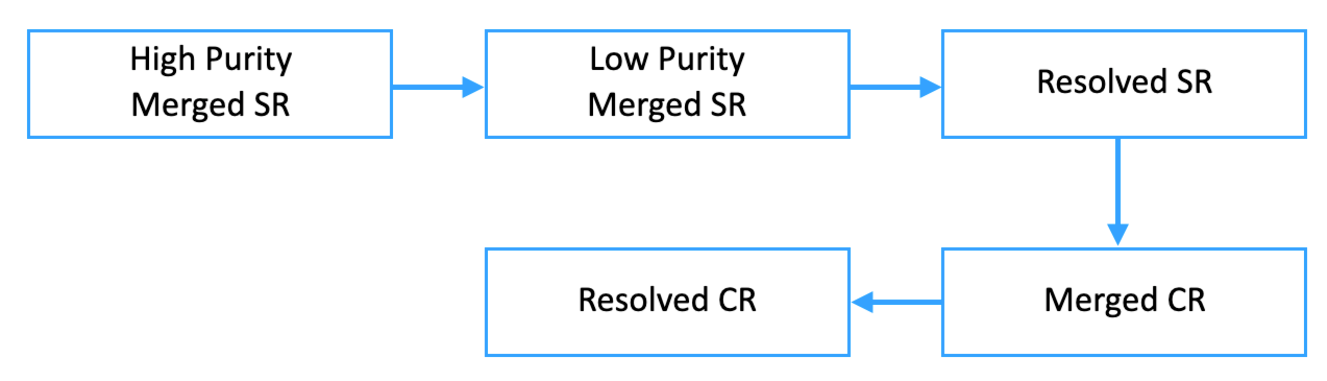
\includegraphics[width=0.8\textwidth]{figures/order}
    \caption{The order of defining the SR and the CR. The merged SR are defined at first, and the events failed the merged SR selections goes to the selection of the resolved SR, therefore there are no overlapped events within several SR and CRs.}
    \label{fig:order}
\end{figure}

%merged selection
The hadronic decaying $W/Z$ bosons with $p_{T}(W / Z \rightarrow q q) \geq 200 \mathrm{GeV}$, can be reconstructed with jets as large-R jets. This merged region required at least one large-R jet outside of the tagging jets of $|\Delta R|<1.4$. 
The boson-tagger is required to find the reconstructed $W/Z$ bosons and the SRs and CRs are defined. The boson-tagger is based on the three variables; jet mass, $D_2$ and $n_Tracks$. The events passed the boson-tagger working point (WP) at 50$\%$ is categorized to be in the High Purity (HP) Merged SR. The events failed the 50$\%$ WP and passed 80$\%$ goes to the Low Purity (LP) Merged SR. 
The boson-tagger is optimized to maximize the sensitivity to the longitudinally-polarized $W/Z$ bosons. 
The previous study showed that the HPSR is not so sensitive to the fully-transversed aQGC signals, which makes us to keep the LPSR for the aQGC searches. 
%put here the reference!
The Merged region definition is shown in the Figure~\ref{fig:MergedRegion}.
\begin{figure}[ht]
    \centering
    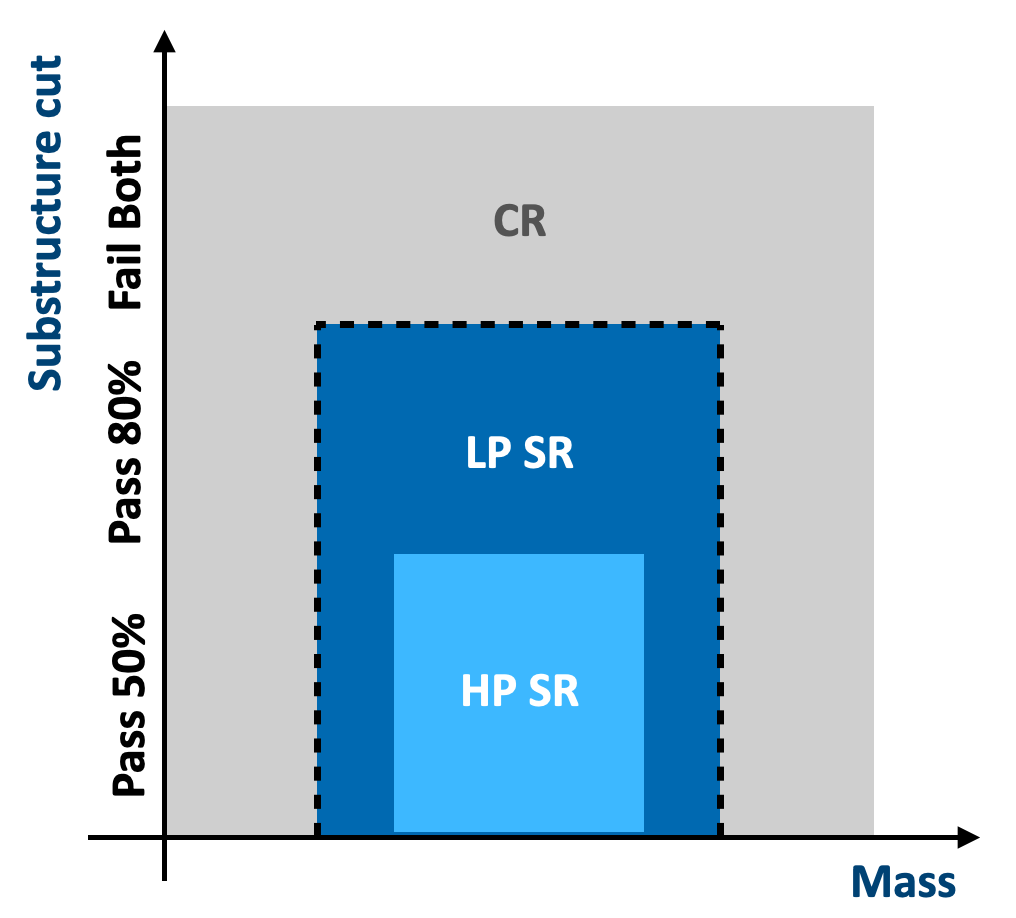
\includegraphics[width=0.6\textwidth]{figures/MergedRegion}
    \caption{The selection of the merged SR and CR are shown. The CR definition is what was changed from the previous round of the analysis, in order to fulfill the requirement to derive the scale factors.}
    \label{fig:MergedRegion}
\end{figure}


%resolved selection
For the bosons with the lower $p_T$ ranges, the boson decays into the two well-separated jets. This is cotegorized as resolved region, with having two signal jets. The two small-R jets are selected from the rest of the jets after tagging jets selection. The leading signal jet is required to be $p_T$ > 40~GeV. The events are categorized to the resolved SR when pass the mass window of 64 < $m_{jj}$ 106~GeV. Figure~\ref{fig:MVHadResSR} shows that the reconstructed boson peak.
%This signal-jet selecting strategy is changed from the previous round of the analysis..
%VBS selection and top veto cut
The event selection is applied to enhance the VBS topology. After categorization the invariant mass of the two tagging jets ($\mathrm{m}_{\mathrm{jj}}^{\text {tag }}$) is greater than $400 \mathrm{GeV}$.
The additional cut is applied to suppress the top contributions for example tZb diagram from the diagram with the Figure~\ref{fig:feynmantZb} included in the signal sample. The top contribution is not the VBS diagrams, while we cannot separate this diagram in the gauge invariant way. Therefore we decided to reconstruct the top mass with the two signal jets and the third jet which forms the three-jet mass, $m_{jjj}$, the closest to the Top mass (172.76~GeV). The $m_{jjj}$ with events with each truth particles is shown, and the modeling plot is also shown in Figure~\ref{fig:2leptopMass}. 
\begin{figure}[ht]
    \begin{center}
        \subfigure[$\text{top mass peak}$]{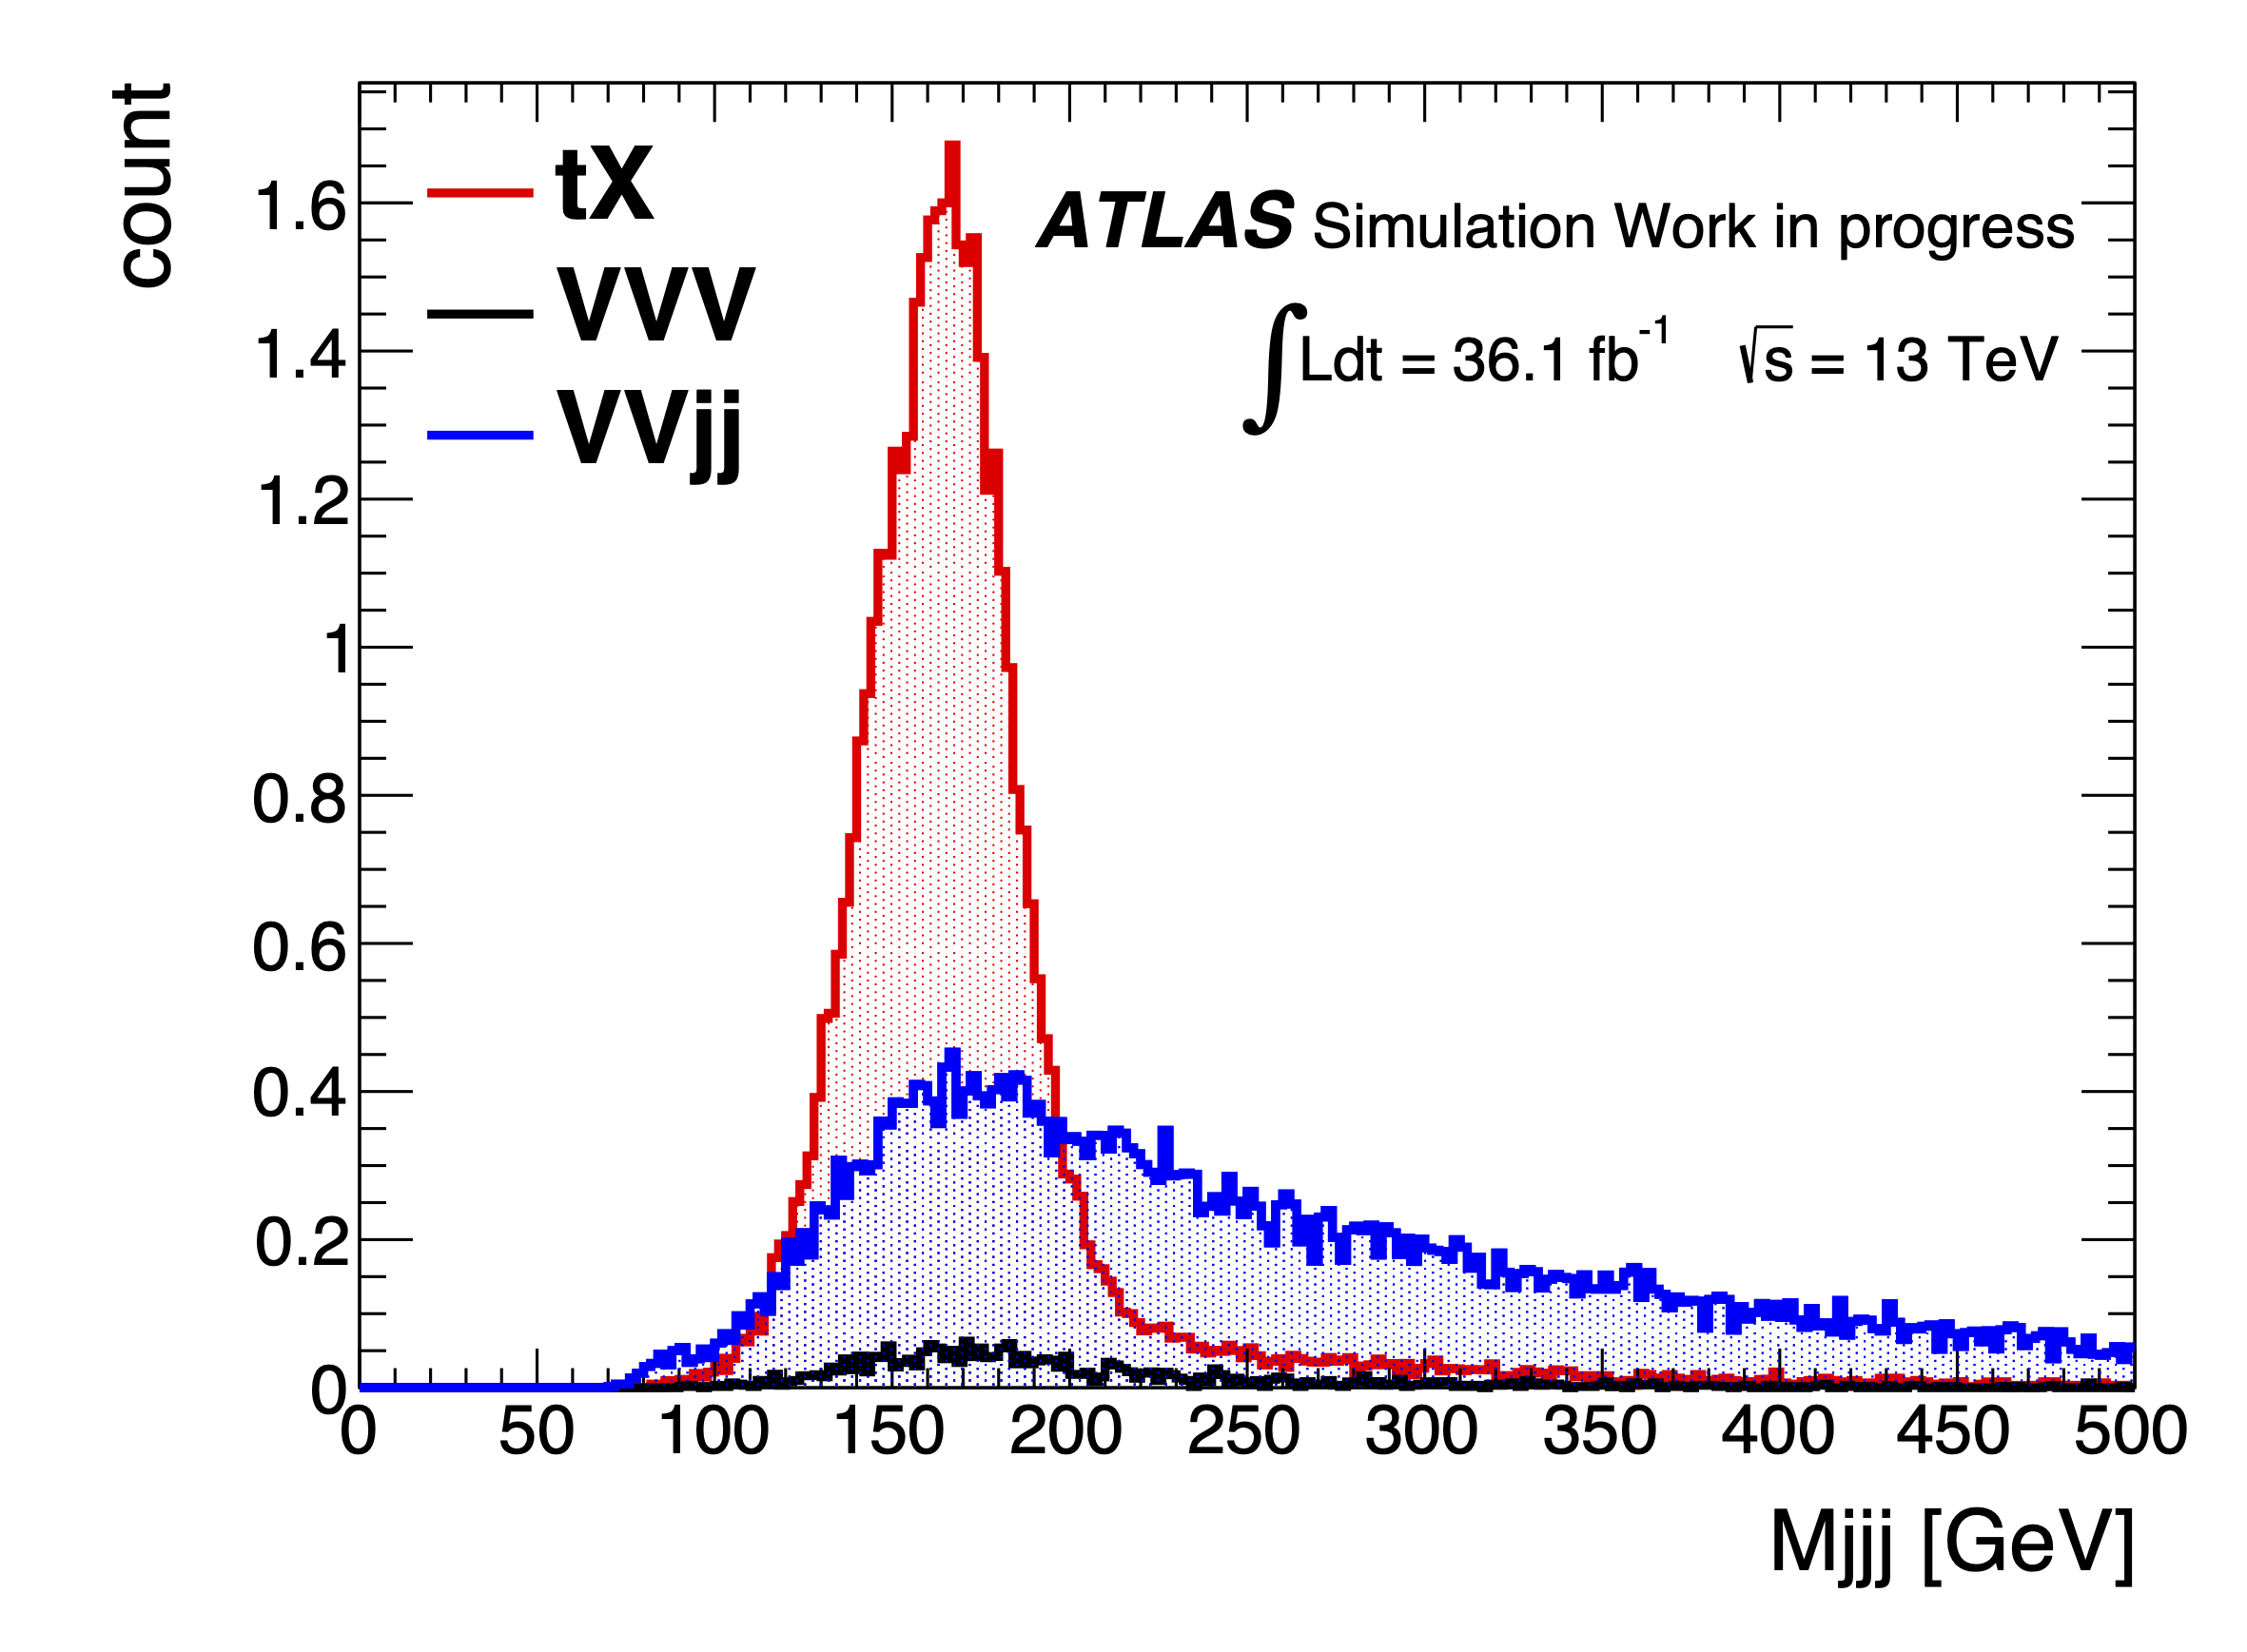
\includegraphics[width=0.3\textwidth]{figures/2lep/topMass/WZjjtopMasspeak}}
        \subfigure[$\text{top mass in CRVjet}$]{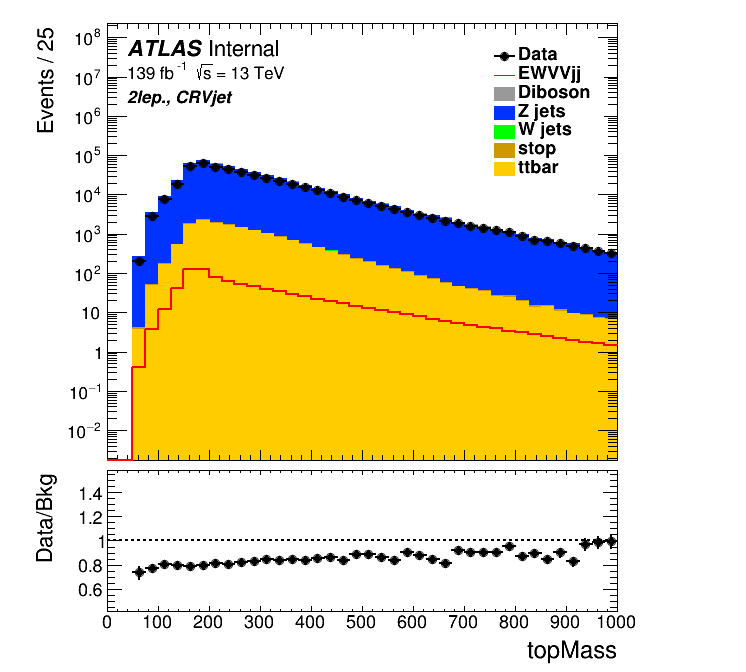
\includegraphics[width=0.3\textwidth]{figures/2lep/dataMC/C_0ptag2pjet_0ptv_CRVjet_topMass_Log}}
        \caption{ Mass of 3 jets in the 2-lepton channel CRVjet.}
        \label{fig:2leptopMass}
    \end{center}
\end{figure}

%Control regions
There are control regions (CR) are defined to constrain the normalization of the backgrounds. The CRs for the $Z$+jets, $W$+jets, and $t\bar{t}$ events are defined here.
%V+jets CR
For the merged CRs, the V+jets CRs are defined for the events failing the 80$\%$ WP of the boson tagger. Resolved CRs are defined with using the mass sideband. It is defined with the same event selection as the resolved SR but outside the mass window, which is $50<m_{i i}<64 \mathrm{GeV}$, or $m_{i i}>106 \mathrm{GeV}$.
%top CR
Top CR is defined only for 1-lepton channel, by requiring at least one b-tagged instead of b-veto. This Top CR is used for constraining the normalization of the $t\bar{t}$ control region. 

The summaries of the selections applied in each channel are shown here in tables.
\ref{tab:0lep_merged}-\ref{tab:0lep_resolved}
\ref{tab:1lep_merged}-\ref{tab:1lep_resolved}
\ref{tab:2lep_merged}-\ref{tab:2lep_resolved}

%%% 0-lepton channel
\begin{table}[ht!]
\small
\caption{A summary of regions event selection for 0-lepton channel in the merged regime.}
\label{tab:0lep_merged}
\begin{center}
\resizebox{\textwidth}{!}{
\begin{tabular}{|l|l|c|c|c|}
\hline
\multicolumn{2}{|l|}{\multirow{2}{*}{Selection}} & \multicolumn{2}{c|}{SR}  &  $V$ CR \\
\cline{3-5}
\multicolumn{2}{|l|}{} & HP & LP & inclusive \\
\hline
\multirow{3}{*}{$Z \to \nu\nu$}  &  Number of Loose leptons & \multicolumn{3}{c|}{0} \\
\cline{2-5}
    & \met                                     & \multicolumn{3}{c|}{ > 200 GeV }                  \\
\cline{2-5}
    & \mpt                                     & \multicolumn{3}{c|}{ > 50 GeV}                    \\
\hline

\multirow{3}{*}{anti-QCD}  & min($\Delta\Phi$(\met,small-R jets))     & \multicolumn{3}{c|}{ $> \pi/6$} \\
\cline{2-5}
    & $\Delta\Phi$(\met,\mpt)                  & \multicolumn{3}{c|}{ $< \pi/2$}                   \\
\cline{2-5}
    & $\Delta\phi(\met, Sig-J)$                & \multicolumn{3}{c|}{ $> \pi/9$}                   \\
\hline
\multirow{3}{*}{VBS jets candidates} & Leading Tag jet \pt & \multicolumn{3}{c|}{ $>30\,\GeV$ } \\
\cline{2-5}
                          & Subleading Tag jet \pt & \multicolumn{3}{c|}{ $>30\,\GeV$ }\\
\cline{2-5}
                          & $m_{jj}$ & \multicolumn{3}{c|}{ $> 400 \GeV$ } \\
\hline
\multirow{2}{*}{$W/Z \to J$} & Num of large-R jets & \multicolumn{3}{c|}{$\geq 1$} \\
\cline{2-5}
& 3-Var Tagger & pass50WP & pass80WP \&\& !pass50WP & fail80WP \\
\hline
\end{tabular}
}
\end{center}
\end{table}


\begin{table}[ht!]
\small
\caption{A summary of regions event selection for 0-lepton channel in the resolved regime.}
\label{tab:0lep_resolved}
\begin{center}
\resizebox{\textwidth}{!}{
\begin{tabular}{|l|l|c|c|}
\hline
\multicolumn{2}{|l|}{Selection} & SR  & $V$ CR \\
\hline
\multirow{3}{*}{$Z \to \nu\nu$}  &  Number of Loose leptons & \multicolumn{2}{c|}{0} \\
\cline{2-4}
    & \met                                     & \multicolumn{2}{c|}{ > 200 GeV }                  \\
\cline{2-4}
    & \mpt                                     & \multicolumn{2}{c|}{ > 50 GeV}                    \\
\hline

\multirow{3}{*}{anti-QCD}  & min($\Delta\Phi$(\met,small-R jets))     & \multicolumn{2}{c|}{ $> \pi/6$} \\
\cline{2-4}
    & $\Delta\Phi$(\met,\mpt)                  & \multicolumn{2}{c|}{ $< \pi/2$}                   \\
\cline{2-4}
    & $\Delta\phi(\met, Sig-J)$                & \multicolumn{2}{c|}{ $> \pi/9$}                   \\
\hline
\multirow{3}{*}{VBS jets candidates} & Leading Tag jet \pt & \multicolumn{2}{c|}{ $>30\,\GeV$ } \\
\cline{2-4}
                          & Subleading Tag jet \pt & \multicolumn{2}{c|}{ $>30\,\GeV$ }\\
\cline{2-4}
                          & $m_{jj}$ & \multicolumn{2}{c|}{ $> 400 \GeV$ } \\
\hline
\multirow{4}{*}{$W/Z \to jj$} & Num of signal small-R jets & \multicolumn{2}{c|}{2} \\
\cline{2-4}
              & Leading signal jet \pt & \multicolumn{2}{c|}{ $>40\,\GeV$ }\\
\cline{2-4}
              & Subleading signal jet \pt & \multicolumn{2}{c|}{ $>20\,\GeV$ }\\
\cline{2-4}
              &$Z \to q\bar{q}$ and $W \to q\bar{q}$     &   $64 < m_{jj} < 106 \gev$ & $50<m_{jj}<64 \,GeV$ or $m_{jj}>106$ \\
\hline
VBS enhancing & $m_{jjj}$ & \multicolumn{2}{c|}{ $>220$~GeV} \\
\hline
\end{tabular}
}
\end{center}
\end{table}

%%% 1-lepton channel
\begin{table}[t]
  \caption{A summary of regions event selection for 1-lepton channel in the resolved regime.}
\label{tab:1lep_resolved}
\begin{center}
\resizebox{\textwidth}{!}{
\begin{tabular}{|l|l|c|c|c|}
\hline
\multicolumn{2}{|l|}{cuts} & SR & $W$ CR (WR) & \ttbar CR (TR) \\
\hline
\multirow{4}{*}{$W\rightarrow \ell\nu$ } & Number of Tight leptons & \multicolumn{3}{c|}{ 1 } \\
\cline{2-5}
&Number of Loose leptons & \multicolumn{3}{c|}{ 0 }  \\
\cline{2-5}
&\met & \multicolumn{3}{c|}{ $>80\,\GeV$ } \\
\cline{2-5}
&$\pt(\ell)$ & \multicolumn{3}{c|}{ $>30\,\GeV$ } \\
\hline
\multirow{3}{*}{VBS jets candidates} & Leading Tag jet \pt & \multicolumn{3}{c|}{ $>30\,\GeV$ } \\
\cline{2-5}
                          & Subleading Tag jet \pt & \multicolumn{3}{c|}{ $>30\,\GeV$ }\\
\cline{2-5}
                          & $m_{jj}$ & \multicolumn{3}{c|}{ $> 400 \GeV$ } \\
\hline
\multirow{4}{*}{$W/Z\rightarrow jj$ } & Number of small-R jets & \multicolumn{3}{c|}{ $\geq 4$ } \\ %$\geq 2$ & $\geq 2$ & $\geq 2$  \\
\cline{2-5}
& Leading jet \pt & \multicolumn{3}{c|}{ $>40$~GeV}\\
\cline{2-5}
& Subleading jet \pt & \multicolumn{3}{c|}{ $>20$~GeV}\\
\cline{2-5}
 &$Z \to q\bar{q}$ and $W \to q\bar{q}$     &   $64 < m_{jj} < 106 \gev$ & $50<m_{jj}<64 \,GeV$ or $m_{jj}>106$ & $64 < m_{jj} < 106 \gev$ \\
\hline
Top veto &  Number of additional $b$-tagged jets & \multicolumn{2}{c|}{0} & $\geq 1$ \\
\hline
VBS enhancing & $m_{jjj}$ & \multicolumn{3}{c|}{ $>220$~GeV} \\
\hline
\end{tabular}
}
\end{center}
\end{table}

\begin{table}[t]
\caption{A summary of regions event selection for 1-lepton channel in the merged regime.}
\label{tab:1lep_merged}
\begin{center}
\resizebox{\textwidth}{!}{
\begin{tabular}{|l|l|c|c|c|c|c|}
\hline
\multicolumn{2}{|l|}{\multirow{2}{*}{Selection}} & \multicolumn{2}{c|}{SR}  &  $W$ CR (WR)  & \multicolumn{2}{c|}{$t\bar{t}$ CR (TR)} \\
\cline{3-7}
\multicolumn{2}{|l|}{} & HP & LP & incl & HP & LP \\
\hline
\multirow{4}{*}{$W\rightarrow \ell\nu$} & Num of Tight leptons & \multicolumn{5}{c|}{ 1 } \\
\cline{2-7}
&Num of Loose leptons & \multicolumn{5}{c|}{ 0 }  \\
\cline{2-7}
&\vphantom{\Large B} \met & \multicolumn{5}{c|}{ $>80\,\GeV$ } \\
\cline{2-7}
&$\pt(\ell)$ & \multicolumn{5}{c|}{ $>30\,\GeV$ } \\
\hline
\multirow{3}{*}{VBS jets candidates} & Leading Tag jet \pt & \multicolumn{5}{c|}{ $>30\,\GeV$ } \\
\cline{2-7}
                          & Subleading Tag jet \pt & \multicolumn{5}{c|}{ $>30\,\GeV$ }\\
\cline{2-7}
                          & $m_{jj}$ & \multicolumn{5}{c|}{ $> 400 \GeV$ } \\
\hline
\multirow{2}{*}{$W/Z\rightarrow J$} & Num of large-$R$ jets & \multicolumn{5}{c|}{ $\geq 1$ } \\
\cline{2-7}
& 3-Var Tagger & pass50WP & pass80WP \&\& !pass50WP & fail80WP & pass50WP & pass80WP \&\& !pass50WP \\
%& \vphantom{\Large B} $D_2/n_{Tracks}$ cut & pass & fail & pass & fail & pass & fail \\
%\cline{2-8}
%& $W/Z$ mass window cut & pass & pass & fail & fail & pass & pass\\
\hline
Top veto & Num of $b$-tagged jets outside of large-R jet & \multicolumn{3}{c|}{0} & \multicolumn{2}{c|}{$\geq 1$} \\
\hline
\end{tabular}
}
\end{center}
\end{table}

%%% 2-leptons channel
\begin{table}[ht!]
\small
\caption{A summary of regions event selection for 2-lepton channel in the merged regime.}
\label{tab:2lep_merged}
\begin{center}
\resizebox{\textwidth}{!}{
\begin{tabular}{|l|l|c|c|c|}
\hline
\multicolumn{2}{|l|}{\multirow{2}{*}{Selection}} & \multicolumn{2}{c|}{SR}  &  $Z$ CR \\
\cline{3-5}
\multicolumn{2}{|l|}{} & HP & LP & incl \\
\hline
\multirow{6}{*}{$Z \to \ell\ell$}  &  Number of Loose leptons & \multicolumn{3}{c|}{2} \\
\cline{2-5}
                          & Same flavor &  \multicolumn{3}{c|}{yes} \\
\cline{2-5}
                          & Leading lepton \pt  & \multicolumn{3}{c|}{$>27\,\GeV$} \\
\cline{2-5}
                          & Subleading lepton \pt  & \multicolumn{3}{c|}{$>27\,\GeV$} \\
\cline{2-5}
                          & \multirow{2}{*}{dilepton invariant mass} & \multicolumn{3}{c|}{$ 83 < m_{ee} < 99 \gev$} \\
                          &  & \multicolumn{3}{c|}{$-0.01170\ptll+85.63 < m_{\mu\mu} < 0.01850\ptll+94.00 \gev$} \\
\cline{2-5}
                          & Opposite sign &  \multicolumn{3}{c|}{For $\mu\mu$ channel only} \\
\hline
\multirow{3}{*}{VBS jets candidates} & Leading Tag jet \pt & \multicolumn{3}{c|}{ $>30\,\GeV$ } \\
\cline{2-5}
                          & Subleading Tag jet \pt & \multicolumn{3}{c|}{ $>30\,\GeV$ }\\
\cline{2-5}
                          & $m_{jj}$ & \multicolumn{3}{c|}{ $> 400 \GeV$ } \\
\hline
\multirow{2}{*}{$W/Z \to J$} & Num of large-R jets & \multicolumn{3}{c|}{$\geq 1$} \\
\cline{2-5}
& 3-Var Tagger & pass50WP & pass80WP \&\& !pass50WP & fail80WP \\
\hline
\end{tabular}
}
\end{center}
\end{table}

\begin{table}[ht!]
\small
\caption{A summary of regions event selection for 2-lepton channel in the resolved regime.}
\label{tab:2lep_resolved}
\begin{center}
\resizebox{\textwidth}{!}{
\begin{tabular}{|l|l|c|c|}
\hline
\multicolumn{2}{|l|}{Selection} & SR  & $Z$ CR \\
\hline
\multirow{6}{*}{$Z \to \ell\ell$}  &  Number of Loose leptons & \multicolumn{2}{c|}{2} \\
\cline{2-4}
                          & Same flavor &  \multicolumn{2}{c|}{yes} \\
\cline{2-4}
                          & Leading lepton \pt  & \multicolumn{2}{c|}{$>27\,\GeV$} \\
\cline{2-4}
                          & Subleading lepton \pt  & \multicolumn{2}{c|}{$>27\,\GeV$} \\
\cline{2-4}
                          & \multirow{2}{*}{dilepton invariant mass} & \multicolumn{2}{c|}{$ 83 < m_{ee} < 99 \gev$} \\
                          & & \multicolumn{2}{c|}{$-0.01170\ptll+85.63 < m_{\mu\mu} < 0.01850\ptll+94.00 \gev$} \\
\cline{2-4}
                          & Opposite sign &  \multicolumn{2}{c|}{For $\mu\mu$ channel only} \\
\hline
\multirow{3}{*}{VBS jets candidates} & Leading Tag jet \pt & \multicolumn{2}{c|}{ $>30\,\GeV$ } \\\cline{2-4}
                          & Subleading Tag jet \pt & \multicolumn{2}{c|}{ $>30\,\GeV$ }\\
\cline{2-4}
                          & $m_{jj}$ & \multicolumn{2}{c|}{ $> 400 \GeV$ } \\
\hline
\multirow{4}{*}{$W/Z \to jj$} & Num of signal small-R jets & \multicolumn{2}{c|}{2} \\
\cline{2-4}
              & Leading signal jet \pt & \multicolumn{2}{c|}{ $>40\,\GeV$ }\\
\cline{2-4}
              & Subleading signal jet \pt & \multicolumn{2}{c|}{ $>20\,\GeV$ }\\
\cline{2-4}
              &$Z \to q\bar{q}$ and $W \to q\bar{q}$     &   $64 < m_{jj} < 106 \gev$ & $50<m_{jj}<64 \,GeV$ or $m_{jj}>106$ \\
\hline
VBS enhancing & $m_{jjj}$ & \multicolumn{2}{c|}{ $>220$~GeV} \\
\hline
\end{tabular}
}
\end{center}
\end{table}
